\documentclass[a4paper,12pt]{article}

\usepackage{amsmath}
\usepackage{float}
\usepackage{graphicx}
\usepackage{listings}

\title{Assignment 2: Fourier Transform and Frequency Filtering}
\author{Aleksandr Jan Smoliakov}
\date{2024--11--07}

\begin{document}

\maketitle

\section{Introduction}

The Fourier Transform is a fundamental tool in signal and image processing, providing powerful techniques for analyzing frequency components of signals and enabling manipulations in both spatial and frequency domains. This report explores various aspects of the Fourier Transform and its applications in image processing tasks, including frequency analysis, filtering, and noise removal.

The report is structured into four sections, each addressing a specific objective.

In \textbf{Fourier Transform and Inverse Fourier Transform}, we examine the process of applying the Fourier Transform and then its inverse to images without making any alterations to their frequency content. This section serves as a foundational step to understand the transformation between spatial and frequency domains.

In \textbf{Fourier Transform of Generated Images}, we investigate the Fourier Transform of synthetically generated images to the demonstrate the relationship between spatial patterns and their frequency-domain counterparts. By analyzing the Fourier spectra of different patterns, we gain insights into how spatial features are represented in the frequency domain.

In \textbf{Filtering in Frequency Space}, we implement frequency-domain filters, including Ideal, Butterworth, and Gaussian filters. Furthermore, we apply image filtering techniques in both spatial and frequency domains to compare their effects on images. This section highlights the advantages and limitations of frequency-based filtering in manipulating image features.

Finally, \textbf{Image Restoration - Noise Removal} focuses on image restoration through noise removal. We demonstrate the removal of periodic noise from images by applying frequency-based filtering techniques. This section shows the effectiveness of frequency filters in eliminating specific noise patterns from images.

\newpage

\tableofcontents

\newpage

\section{Fourier Transform and Inverse Fourier Transform}

In this section, we will apply the Fourier Transform and Inverse Fourier Transform to an input image without any modifications. The goal is to transform the image to the frequency domain and then reconstruct it back to the spatial domain to verify the correctness of the transformations.

\subsection{Theoretical Background}

\subsubsection{Fourier Transform}

The Fourier Transform is a mathematical operation that decomposes a signal into its constituent sinusoidal components. In image processing, the Fourier Transform is used to analyze the frequency content of images, identifying patterns, textures, and structures in the spatial domain. The Fourier Transform of a signal \( f(x) \) is defined as:

\begin{equation}
    F(u) = \int_{-\infty}^{\infty} f(x) \cdot e^{-j 2 \pi u x} \, dx
\end{equation}

where:

\begin{itemize}
    \item \( F(u) \) is the Fourier Transform of the signal.
    \item \( f(x) \) represents the signal in the spatial domain.
    \item \( u \) is the frequency component.
\end{itemize}

The Fourier Transform converts a signal from the spatial domain to the frequency domain, providing information about the amplitude and phase of each frequency component present in the signal.

\subsubsection{Discrete Fourier Transform (DFT)}

In digital image processing, signals are represented as discrete data points.

For a greyscale 2D image \( f(x, y) \) of size \( M \times N \) pixels, which is a discrete signal, the \textbf{Discrete Fourier Transform (DFT)} algorithm can be used to transform the image from the spatial domain to the frequency domain. The DFT is defined as:

\begin{equation}
    F(u, v) = \sum_{x=0}^{M-1} \sum_{y=0}^{N-1} f(x, y) \cdot e^{-j 2 \pi \left(\frac{ux}{M} + \frac{vy}{N} \right)}
\end{equation}

where:

\begin{itemize}
    \item \( F(u, v) \) is the DFT result in the frequency domain.
    \item \( f(x, y) \) represents the pixel intensity at position \( (x, y) \).
    \item \( u \) and \( v \) are frequency components in the x and y directions, respectively.
    \item \( M \) and \( N \) are the dimensions of the image.
\end{itemize}

The DFT decomposes an image into sinusoidal frequency components, with \( F(u, v) \) representing the amplitude and phase of each frequency component at coordinates \( (u, v) \) in the frequency domain. Understanding the Fourier spectrum allows us to identify dominant frequencies and orientations in patterns.

\subsubsection{Inverse Fourier Transform}

The \textbf{Inverse Discrete Fourier Transform (IDFT)} returns the transformed data back to the spatial domain:

\begin{equation}
    f(x, y) = \frac{1}{M \cdot N} \sum_{u=0}^{M-1} \sum_{v=0}^{N-1} F(u, v) \cdot e^{j 2 \pi \left(\frac{ux}{M} + \frac{vy}{N} \right)}
\end{equation}
    
\subsection{Methodology}

The list below outlines the step-by-step process for implementing the Fourier Transform on an image, transforming it to the frequency domain, and then reconstructing it using the Inverse Fourier Transform:

\begin{enumerate}
    \item \textbf{Input Image}:
        We start with a greyscale image with dimensions \( M \times N \). This is the base image that will be transformed.
    \item \textbf{Padding the Image to 2M x 2N}:
        The image is padded to twice its original dimensions, the resulting dimensions become \( 2M \times 2N \). The original image stays in the upper-left corner, and the remaining space is filled with zeros. This padding helps in analyzing frequency components by increasing the resolution in the frequency domain and thus avoiding wraparound artifacts in the Fourier Transform.
    \item \textbf{Shifting for Periodicity}:
        To prepare the image for the Fourier Transform, we apply a shift operation by alternating the sign of every second pixel. Mathematically, this involves multiplying the image by \( (-1)^{x + y} \), where \( x \) and \( y \) represent the pixel coordinates. This operation centers the low-frequency components by aligning the image's origin with the center of the Fourier spectrum.
    \item \textbf{Discrete Fourier Transform (DFT)}:
        2D Discrete Fourier Transform is then applied to the shifted image. In Python, this transformation is performed by the \texttt{numpy.fft.fft2()} function, generating complex values that represent the amplitude and phase of each frequency component. This step provides a matrix \( F(u, v) \) where each element corresponds to a specific frequency in the image. The Fourier spectrum is then visualized by taking \( \log(1 + \text{abs}(F(u, v))) \) to reduce the contrast and enhance visibility of frequency components.
    \item \textbf{Inverse Discrete Fourier Transform (IDFT)}:
        The inverse Fourier Transform is computed on \( F(u, v) \). The resulting data is shifted back to its original configuration (reversing the initial shift). In Python, the IDFT is performed by \texttt{numpy.fft.ifft2()}.@
        This reconstructed data represents the image in the spatial domain.
    \item \textbf{Extraction of the Upper-Left Quadrant}:
        Finally, the upper-left quadrant of the IDFT output is extracted, resizing it to the original image dimensions \( M \times N \). If the Fourier Transform and Inverse Fourier Transform are implemented correctly, this quadrant should closely resemble the original image, indicating a successful transformation and reconstruction.
\end{enumerate}

\subsection{Results}

Terminal command to run the Fourier Transform and Inverse Fourier Transform on an input image:

\begin{lstlisting}[language=bash]
$ python python/main.py two-way-fourier \
    data/input/Fig0507\(a\)\(ckt-board-orig\).tif
\end{lstlisting}

Figure~\ref{fig:two-way-fourier} illustrates the intermediate stages of the Fourier Transform and Inverse Fourier Transform on the input image.

\begin{figure}[hbtp]
    \begin{tabular}{cc}
        \includegraphics[width=0.45\textwidth]{data/output/two_way_fourier/01_original_image.png} &
        \includegraphics[width=0.45\textwidth]{data/output/two_way_fourier/02_padded_image.png} \\
        (a) Original Image & (b) Padded Image \\
        \includegraphics[width=0.45\textwidth]{data/output/two_way_fourier/03_shifted_for_periodicity.png} &
        \includegraphics[width=0.45\textwidth]{data/output/two_way_fourier/04_dft.png} \\
        (c) Shifted for Periodicity & (d) Magnitude of DFT in Frequency Domain \\
        \includegraphics[width=0.45\textwidth]{data/output/two_way_fourier/05_inverse_dft.png} &
        \includegraphics[width=0.45\textwidth]{data/output/two_way_fourier/07_upper_left_quadrant.png} \\
        (e) Magnitude of Inverse DFT & (f) Upper-Left Quadrant \\
    \end{tabular}
    \caption{\label{fig:two-way-fourier} Stages of the Fourier Transform and Inverse Fourier Transform.}
\end{figure}

The reconstructed image (f) closely resembling the original image (a). Thus, the Fourier Transform and Inverse Fourier Transform have been successfully applied to the input image. Additionally, the Fourier spectrum (d) shows the distribution of frequency components in the image, with brighter low-frequency components concentrated near the center, and high-frequency components at the edges. The repeated vertical and horizontal lines in the frequency spectrum indicate the presence of periodic patterns in the image.

\newpage

\section{Fourier Transform of Generated Images}

In this section, we will generate synthetic images with distinct spatial patterns and analyze their Fourier spectra. By examining the frequency components of these patterns, we can observe how different spatial features look in the frequency domain.

For this experiment, we will generate greyscale \(256 \times 256\) pixel images with three distinct spatial patterns:

\begin{itemize}
    \item 2D Sine Wave Pattern
    \item Vertical Lines Pattern
    \item Checkerboard Pattern
\end{itemize}

For each pattern, we will describe the expected Fourier spectra. Then the generated images will be DFT-transformed to the frequency domain, and the Fourier spectra will be visualized to verify the expected frequency components.

\subsection{Methodology}

Each pattern is generated and transformed following these steps:

\begin{enumerate}
    \item \textbf{Image Generation}:
        A greyscale 2D image \(256 \times 256\) pixels is generated with the desired spatial pattern.
    \item \textbf{Discrete Fourier Transform (DFT)}:
        The 2D Discrete Fourier Transform (\texttt{numpy.fft.fft2}) is used to convert the generated image to the frequency domain. The Fourier spectrum is shifted to center the low-frequency components using \texttt{numpy.fft.fftshift}, making it easier to visualize the frequency distribution.
    \item \textbf{Visualization of Fourier Spectrum}:
        The magnitude of the Fourier Transform is computed, and the logarithm of the magnitude (plus 1 to avoid \(\log(0)\)) is taken to reduce the intensity range and enhance visibility of frequency components. The Fourier spectrum is then displayed alongside the generated image for comparison.
\end{enumerate}

\subsubsection{2D Sine Wave Pattern}
A 2D sine wave consists of two same-frequency sinusoidal patterns oscillating in the x and y directions. The image is generated by multiplying a sine wave on both the x and y axes. The signal is then scaled to the range [0, 1] to create a greyscale image.

\textbf{Generation}: The pattern is generated by setting pixel intensities based on a cosine function with a chosen frequency in the x and y directions:

\[
    f(x, y) = \frac{1}{2} \cdot \left(\cos(\alpha \cdot x) \cdot \cos(\alpha \cdot y) + 1\right)
\]
where \( \alpha \) = 2\(\pi\) / size, and \( size \) defines the wavelength of the sine wave.

\textbf{Expected Fourier Spectrum}: Since the Fourier Transform itself reduces a signal to a sum of sinusoids, we expect that this image will be reduced to two sine waves. The Fourier spectrum should display a bright spot at the frequency coordinates used to create the pattern (\( \alpha, \alpha \)), and three other spots in the negative frequency quadrants.

\subsubsection{Vertical Line Pattern}
A pattern of vertical lines represents high-frequency components in the horizontal direction, with zero variation along the vertical axis.

\textbf{Generation}: The pattern consists of vertical lines with a specific spatial frequency along the x-axis. The pattern can be created by setting pixel values based on:

\[
    f(x, y) = \frac{1}{2} \cdot \left( \text{sign}(\sin(\alpha \cdot x)) + 1 \right)
\]
where \( \alpha \) = 2\(\pi\) / size, and \( size \) controls the width of the two vertical lines.

\textbf{Expected Fourier Spectrum}: Since this pattern has no signal in the vertical direction, we expect that the entire Fourier spectrum will be concentrated along the horizontal axis. Since the vertical lines are essentially a square wave in the horizontal direction, the Fourier spectrum should show to symmetric bright spots at the frequency of the vertical lines \( \alpha \), with dimmer spots at their odd harmonics (3\(\alpha\), 5\(\alpha\), etc.).

\subsubsection{Checkerboard Pattern}
The checkerboard pattern contains alternating black and white squares. The sharp boundaries of the squares introduce high-frequency components along both axes. We expect that the Fourier spectrum of this pattern should display a grid of high-intensity points, similar to the vertical lines pattern but on both axes.

\textbf{Generation}: The checkerboard pattern alternates between maximum and minimum values, thus creating a chessboard (or checkerboard) like grid. This pattern can be represented as:

\[
    f(x, y) = \frac{1}{2} \cdot \left( \text{sign}(\sin(\alpha \cdot x) \cdot \sin(\alpha \cdot y)) + 1 \right)
\]
where \( \alpha \) = 2\(\pi\) / size, and \( size \) defines the size of a 2 \(\times\) 2 square.

\textbf{Expected Fourier Spectrum}: A checkerboard pattern is essentially a 2D version of the vertical lines pattern. In other words, the signal on both axes is a square wave, and we expect to see a grid-like structure in the Fourier spectrum. We expect to see high-intensity points at the frequency of the squares \( \alpha, \alpha \), and their odd harmonics (3\(\alpha\), 5\(\alpha\), etc.).

\subsection{Results}

\subsubsection{2D Sine Wave Pattern}

Terminal command to generate the Sine Wave Pattern image and its Fourier spectrum:

\begin{lstlisting}[language=bash]
$ python python/main.py image-generation \
    sine --size 256
\end{lstlisting}

Here, the \texttt{size} parameter controls the wavelength (in pixels) of the sine wave pattern.

In Figure~\ref{fig:sine-wave-pattern}, the 2D Sine Wave Pattern image and its Fourier spectrum are displayed.

\begin{figure}
    \begin{tabular}{cc}
        \includegraphics[width=0.45\textwidth]{data/output/image_generation/sine/01_generate_image.png} &
        \includegraphics[width=0.45\textwidth]{data/output/image_generation/sine/03_shifted_dft.png} \\
        (a) Generated Image & (b) Fourier Spectrum (Shifted) \\
    \end{tabular}
    \caption{\label{fig:sine-wave-pattern} Sine Wave Pattern and its Fourier Spectrum.}
\end{figure}

The Fourier spectrum shows four symmetrical peaks centered around the origin, corresponding to the low frequency (wavelength = 256px) values used to create the sinusoidal pattern. This verifies that smooth, periodic variations in pixel intensity produce localized frequency components. Additionally, the center pixel of the Fourier spectrum is also bright, indicating the presence of a DC component (mean intensity) in the image. This outcome aligns with the our expectations.

\subsubsection{Vertical Lines Pattern}

Terminal command to generate the Vertical Lines Pattern image and its Fourier spectrum:

\begin{lstlisting}[language=bash]
$ python python/main.py image-generation \
    vertical_lines --size 32
\end{lstlisting}

Here, the \texttt{size} parameter controls the width (in pixels) of two vertical lines in the pattern.

In Figure~\ref{fig:vertical-lines-pattern}, the Vertical Lines Pattern image and its Fourier spectrum are shown.

\begin{figure}
    \begin{tabular}{cc}
        \includegraphics[width=0.45\textwidth]{data/output/image_generation/vertical_lines/01_generate_image.png} &
        \includegraphics[width=0.45\textwidth]{data/output/image_generation/vertical_lines/03_shifted_dft.png} \\
        (a) Generated Image & (b) Fourier Spectrum (Shifted) \\
    \end{tabular}
    \caption{\label{fig:vertical-lines-pattern} Vertical Lines Pattern and its Fourier Spectrum.}
\end{figure}

The Fourier spectrum shows a single dotted pattern along the horizontal axis, indicating the fundamental frequency of the vertical lines. The spectrum also displays dimmer spots at the odd harmonics of the fundamental frequency, representing the higher frequency components. There is also a dot at the center of the Fourier spectrum, indicating the DC component of the image. This outcome aligns with the our expectations.

\subsubsection{Checkerboard Pattern}

Terminal command to generate the Checkerboard Pattern image and its Fourier spectrum:

\begin{lstlisting}[language=bash]
$ python python/main.py image-generation \
    checkerboard --size 32
\end{lstlisting}

Here, the \texttt{size} parameter controls the size (in pixels) of a 2 \(\times\) 2 square in the checkerboard pattern.

In Figure~\ref{fig:checkerboard-pattern}, the Checkerboard Pattern image and its Fourier spectrum are shown.

\begin{figure}
    \begin{tabular}{cc}
        \includegraphics[width=0.45\textwidth]{data/output/image_generation/checkerboard/01_generate_image.png} &
        \includegraphics[width=0.45\textwidth]{data/output/image_generation/checkerboard/03_shifted_dft.png} \\
        (a) Generated Image & (b) Fourier Spectrum (Shifted) \\
    \end{tabular}
    \caption{\label{fig:checkerboard-pattern} Checkerboard Pattern and its Fourier Spectrum.}
\end{figure}

The Fourier spectrum displays a grid-like structure similar to the checkerboard pattern, with high-intensity points at the frequency of the squares and their odd harmonics on both axes. Similarly to the Vertical Lines pattern, here the sharp transitions between black and white squares introduce high-frequency components in the image, producing a grid-like structure in the Fourier spectrum. This outcome aligns with the our expectations.

\newpage

\section{Filtering in Frequency Space}

In this section, we will implement three types of high-pass and low-pass frequency filters: Ideal, Butterworth, and Gaussian filters. Each filter type operates differently in the frequency domain, with their unique characteristics affecting the filtered image. We will demonstrate the frequency masks of these filters, apply them to an image to observe the effects.

\subsection{Theoretical Background}

Frequency filters are essential tools in image processing for enhancing or suppressing specific frequency components. When applied in the frequency domain, these filters modify the Fourier spectrum of an image, affecting the spatial features in the reconstructed image.

High-pass filters emphasize high-frequency components, enhancing edges and fine details in images. They are useful for sharpening images and enhancing contrast.

Low-pass filters, on the other hand, suppress high-frequency components, smoothing the image and reducing noise. They are effective in blurring images and reducing sharp transitions.

\subsubsection{Ideal Filter}

The Ideal filter is the simplest frequency space filter, sharply cutting off frequencies beyond a certain radius.
\begin{itemize}
    \item \textbf{High-Pass Filter:} Blocks low frequencies, passing only high-frequency components.
    \item \textbf{Low-Pass Filter:} Blocks high frequencies, passing only low-frequency components.
\end{itemize}

The Ideal filter is defined as:

\[
    H(u, v) = \begin{cases}
        1 & \text{if } D(u, v) \leq D_0 \\
        0 & \text{if } D(u, v) > D_0
    \end{cases}
\]

Here, \( D(u, v) \) is the distance from the origin in the frequency domain, and \( D_0 \) is the cutoff frequency that determines the radius of the filter.

The Ideal high-pass filter is the complement of the low-pass filter:

\[
    H(u, v) = 1 - H(u, v)
\]

\subsubsection{Butterworth Filter}

The Butterworth filter provides a smoother transition in frequency space, reducing abrupt changes that cause artifacts.
\begin{itemize}
    \item \textbf{High-Pass Filter:} Allows a gradual transition from low to high frequencies.
    \item \textbf{Low-Pass Filter:} Gradually attenuates high frequencies, allowing smoother transitions.
\end{itemize}

The Butterworth filter is defined as:

\[
    H(u, v) = \frac{1}{1 + \left( \frac{D(u, v)}{D_0} \right)^{2n}}
\]

Here, \( D(u, v) \) is the distance from the origin in the frequency domain, \( D_0 \) is the cutoff frequency, and \( n \) is the order of the filter that controls the rate of attenuation.

The Butterworth high-pass filter is the complement of the low-pass filter:

\[
    H(u, v) = 1 - H(u, v)
\]

\subsubsection{Gaussian Filter}

Gaussian filters apply a smooth Gaussian function, which minimizes abrupt frequency changes and provides a natural blur effect.
\begin{itemize}
    \item \textbf{High-Pass Filter:} Gradually attenuates low frequencies with a Gaussian function.
    \item \textbf{Low-Pass Filter:} Gradually attenuates high frequencies, producing smooth, artifact-free images.
\end{itemize}

The Gaussian filter is defined as:

\[
    H(u, v) = e^{-\frac{D^2(u, v)}{2 \sigma^2}}
\]

Here, \( D(u, v) \) is the distance from the origin in the frequency domain, and \( \sigma \) is the standard deviation that controls the spread of the Gaussian function.

The Gaussian high-pass filter is the complement of the low-pass filter:

\[
    H(u, v) = 1 - H(u, v)
\]

\subsubsection{Applying Linear Filters in Frequency and Image Space}

In the previous assignment, we applied linear filters in the spatial domain to process images. Linear filters operate by convolving the image with a kernel to modify pixel values based on the neighbouring pixels.

However, linear filters can also be applied in the frequency domain by transforming both the image and the filter kernel to the frequency domain, multiplying them, and then transforming the result back to the spatial domain.

\subsection{Methodology}

\subsubsection{High-Pass and Low-Pass Filters}

In order to apply the filters in the frequency domain, we will reuse the Fourier Transform and Inverse Fourier Transform functions from the \textbf{Fourier Transform and Inverse Fourier Transform} section. The steps to implement frequency filtering are as follows:

\begin{enumerate}
    \item \textbf{Input Image}:
        We start with a greyscale image with dimensions \( M \times N \). This is the base image that will be transformed.
    \item \textbf{Padding the Image to 2M x 2N}:
        The image is padded to twice its original dimensions, the resulting dimensions become \( 2M \times 2N \). The original image stays in the upper-left corner, and the remaining space is filled with zeros. This padding helps in analyzing frequency components by increasing the resolution in the frequency domain and thus avoiding wraparound artifacts in the Fourier Transform.
    \item \textbf{Shifting for Periodicity}:
        To prepare the image for the Fourier Transform, we apply a shift operation by alternating the sign of every second pixel. Mathematically, this involves multiplying the image by \( (-1)^{x + y} \), where \( x \) and \( y \) represent the pixel coordinates. This operation centers the low-frequency components by aligning the image's origin with the center of the Fourier spectrum.
    \item \textbf{Discrete Fourier Transform (DFT)}:
        2D Discrete Fourier Transform is then applied to the shifted image. In Python, this transformation is performed by the \texttt{numpy.fft.fft2()} function, generating complex values that represent the amplitude and phase of each frequency component. This step provides a matrix \( F(u, v) \) where each element corresponds to a specific frequency in the image. The Fourier spectrum is then visualized by taking \( \log(1 + \text{abs}(F(u, v))) \) to reduce the contrast and enhance visibility of frequency components.
    \item \textbf{Frequency Filtering}:
        The Fourier spectrum is multiplied by a frequency filter mask, which can be an Ideal, Butterworth, or Gaussian filter. The filter mask is designed to attenuate specific frequency components based on the filter type (low-pass or high-pass) and cutoff frequency.
    \item \textbf{Inverse Discrete Fourier Transform (IDFT)}:
        The inverse Fourier Transform is computed on \( F(u, v) \). The resulting data is shifted back to its original configuration (reversing the initial shift). In Python, the IDFT is performed by \texttt{numpy.fft.ifft2()}.@
        This reconstructed data represents the image in the spatial domain.
    \item \textbf{Extraction of the Upper-Left Quadrant}:
        Finally, the upper-left quadrant of the IDFT output is extracted, resizing it to the original image dimensions \( M \times N \). If the Fourier Transform and Inverse Fourier Transform are implemented correctly, this quadrant should closely resemble the original image, indicating a successful transformation and reconstruction.
\end{enumerate}

\subsubsection{Applying Linear Filters in Frequency and Image Space}

We shall apply several types of image filters in the spatial domain and in the frequency domain to compare their effects on images. We will use the same input image and the exact same filter parameters for both spatial and frequency domain filtering to observe the differences in the results. The filters to be applied are:

\begin{itemize}
    \item \textbf{Average Filter}:
        A simple averaging filter that replaces each pixel with the average of its neighbouring pixels.
    \item \textbf{Gaussian Filter}:
        A Gaussian filter that applies a weighted average based on the Gaussian function.
    \item \textbf{Differentiation Filter on the X-axis}:
        A filter that computes the derivative of the image in the x-direction.
\end{itemize}

These filters have been described in the previous assignment and will be reused here.

The steps to apply the filters in the spatial domain are as follows:

\begin{enumerate}
    \item \textbf{Input Image}:
        We start with a greyscale image with dimensions \( M \times N \). This is the base image that will be filtered.
    \item \textbf{Applying the Filter}:
        The selected filter is convolved with the image using the \texttt{scipy.ndimage.convolve} function. The filter kernel is applied to each pixel in the image to modify its intensity based on the neighbouring pixels.
\end{enumerate}

The steps to apply the filters in the frequency domain are exactly the same as in the \textbf{High-Pass and Low-Pass Filters} section, with the only difference being the filter mask used. The filter masks for the Average, Gaussian, and Differentiation filters are computed by transforming the spatial filter kernels to the frequency domain.

Kernel generation for patial domain blurring was implemented and described in the previous assignment and is reused here.

Transforming the filter kernel to the frequency domain involves the following steps:

\begin{enumerate}
    \item \textbf{Padding the Filter Kernel}:
        The filter kernel is padded to the size of the input image to match the dimensions.
    \item \textbf{Shifting for Periodicity}:
        The filter kernel is multiplied by \( (-1)^{x + y} \) to center it for the Fourier Transform.
    \item \textbf{Discrete Fourier Transform (DFT)}:
        2D Discrete Fourier Transform is applied to the filter kernel.
\end{enumerate}

\subsection{Results}

In this section, we will use the raw image from Lesson 6 \texttt{Fig0464(a)(car\_75DPI\_Moire).tif} which is shown in Figure~\ref{fig:car-75dpi-moire}. It's a black and white image of a car with a pronounced moiré pattern. The moiré pattern is not directly related to this exercise, but it provides a good example for filtering in the frequency domain.

\begin{figure}
    \centering
    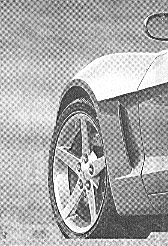
\includegraphics[width=0.33\textwidth]{data/input/Fig0464(a)(car_75DPI_Moire).png}
    \caption{\label{fig:car-75dpi-moire} Raw image of a car with a moiré pattern.}
\end{figure}

Let's apply different types of filters in the frequency domain and observe their effects on the image.

\subsubsection{Ideal Filter}

Terminal command to apply the filters on the raw image:

\begin{lstlisting}[language=bash]
$ python python/main.py frequency-filtering \
    <FILTER_NAME> <IMAGE_PATH> --cutoff <CUTOFF>
\end{lstlisting}

Here:

\begin{itemize}
    \item \texttt{<FILTER\_NAME>} can be either \texttt{ideal\_low\_pass} for a low-pass filter or \texttt{ideal\_high\_pass} for a high-pass filter.
    \item \texttt{<IMAGE\_PATH>} is the path to the input image.
    \item \texttt{--cutoff <CUTOFF>} is the cutoff frequency for the filter, i.e. the \( D_0 \) term in the filter equations. In this case, we use a cutoff of 32.
\end{itemize}

The results of the Ideal Filters on the raw image are shown in Figure~\ref{fig:ideal-filters}.

\begin{figure}[hbtp]
    \begin{tabular}{ccc}
        \includegraphics[width=0.3\textwidth]{data/output/frequency_filtering/ideal_low_pass/01_original_image.png} &
        \includegraphics[width=0.3\textwidth]{data/output/frequency_filtering/ideal_low_pass/03_shifted_for_periodicity.png} &
        \includegraphics[width=0.3\textwidth]{data/output/frequency_filtering/ideal_low_pass/04_dft.png} \\
        (a) Original Image & (b) Shifted for Periodicity & (c) DFT \\
        \includegraphics[width=0.3\textwidth]{data/output/frequency_filtering/ideal_low_pass/05_applied_filter_mask.png} &
        \includegraphics[width=0.3\textwidth]{data/output/frequency_filtering/ideal_low_pass/05_applied_filter.png} &
        \includegraphics[width=0.3\textwidth]{data/output/frequency_filtering/ideal_low_pass/09_upper_left_quadrant.png} \\
        (d) Low-Pass Filter Mask & (e) Filtered DFT & (f) Final Image \\
        \includegraphics[width=0.3\textwidth]{data/output/frequency_filtering/ideal_high_pass/05_applied_filter_mask.png} &
        \includegraphics[width=0.3\textwidth]{data/output/frequency_filtering/ideal_high_pass/05_applied_filter.png} &
        \includegraphics[width=0.3\textwidth]{data/output/frequency_filtering/ideal_high_pass/09_upper_left_quadrant.png} \\
        (g) High-Pass Filter Mask & (h) Filtered DFT & (i) Final Image \\
    \end{tabular}
    \caption{\label{fig:ideal-filters} Results of the Ideal Low-Pass and High-Pass Filters on the raw image.}
\end{figure}

We can observe that the Ideal Filter masks have a very sharp cutoff (d) (g) at the specified frequency. The Ideal Low-Pass Filter (f) smooths the image, reducing the high-frequency components (edges) and the moiré pattern. The Ideal High-Pass Filter (i) removes the zero-frequency component, preserves the edges and successfully captures the moiré pattern, enhancing the fine details in the image. However, in the low-pass filtered image we can observe pronounced \textit{ringing} artifacts around the edges of the car. These artifacts are distinct from the moiré pattern and are a result of the sharp cutoff in the Ideal filter.

Ideal frequency filters are known to introduce artifacts known as ringing artifacts due to the abrupt cutoff in frequencies. This ringing manifests as oscillations around sharp transitions, which are especially noticeable in images with edges.

\subsubsection{Butterworth Filter}

Terminal command to apply the filters on the raw image:

\begin{lstlisting}[language=bash]
$ python python/main.py frequency-filtering \
    <FILTER_NAME> <IMAGE_PATH> --cutoff <CUTOFF> \
    --order <ORDER>
\end{lstlisting}

Here:

\begin{itemize}
    \item \texttt{<FILTER\_NAME>} can be either \texttt{butterworth\_low\_pass} for a low-pass filter or \texttt{butterworth\_high\_pass} for a high-pass filter.
    \item \texttt{<IMAGE\_PATH>} is the path to the input image.
    \item \texttt{--cutoff <CUTOFF>} is the cutoff frequency for the filter, i.e. the \( D_0 \) term in the filter equations. In this case, we use a cutoff of 32.
    \item \texttt{--order <ORDER>} is the order of the Butterworth filter that controls the rate of attenuation, i.e. the \( n \) term in the filter equations. In this case, we use an order of 2.
\end{itemize}

The results of the Butterworth Filters on the raw image are shown in Figure~\ref{fig:butterworth-filters}.

\begin{figure}[hbtp]
    \begin{tabular}{ccc}
        \includegraphics[width=0.3\textwidth]{data/output/frequency_filtering/butterworth_low_pass/01_original_image.png} &
        \includegraphics[width=0.3\textwidth]{data/output/frequency_filtering/butterworth_low_pass/03_shifted_for_periodicity.png} &
        \includegraphics[width=0.3\textwidth]{data/output/frequency_filtering/butterworth_low_pass/04_dft.png} \\
        (a) Original Image & (b) Shifted for Periodicity & (c) DFT \\
        \includegraphics[width=0.3\textwidth]{data/output/frequency_filtering/butterworth_low_pass/05_applied_filter_mask.png} &
        \includegraphics[width=0.3\textwidth]{data/output/frequency_filtering/butterworth_low_pass/05_applied_filter.png} &
        \includegraphics[width=0.3\textwidth]{data/output/frequency_filtering/butterworth_low_pass/09_upper_left_quadrant.png} \\
        (d) Low-Pass Filter Mask & (e) Filtered DFT & (f) Final Image \\
        \includegraphics[width=0.3\textwidth]{data/output/frequency_filtering/butterworth_high_pass/05_applied_filter_mask.png} &
        \includegraphics[width=0.3\textwidth]{data/output/frequency_filtering/butterworth_high_pass/05_applied_filter.png} &
        \includegraphics[width=0.3\textwidth]{data/output/frequency_filtering/butterworth_high_pass/09_upper_left_quadrant.png} \\
        (g) High-Pass Filter Mask & (h) Filtered DFT & (i) Final Image \\
\end{tabular}
\caption{\label{fig:butterworth-filters} Results of the Butterworth Low-Pass and High-Pass Filters on the raw image.}
\end{figure}

Here, the Butterworth filters provide a smoother transition between the passband and stopband (d) (g), without the sharp cutoff of the Ideal filter. The Butterworth Low-Pass Filter (f) effectively smooths the image, reducing the moiré pattern and the edges without introducing ringing artifacts. The Butterworth High-Pass Filter (i) removes the zero-frequency component, enhances the edges and also captures the moiré pattern.

\subsubsection{Gaussian Filter}

Terminal command to apply the filters on the raw image:

\begin{lstlisting}[language=bash]
$ python python/main.py frequency-filtering \
    <FILTER_NAME> <IMAGE_PATH> --cutoff <CUTOFF>
\end{lstlisting}

Here:

\begin{itemize}
    \item \texttt{<FILTER\_NAME>} can be either \texttt{gaussian\_low\_pass} for a low-pass filter or \texttt{gaussian\_high\_pass} for a high-pass filter.
    \item \texttt{<IMAGE\_PATH>} is the path to the input image.
    \item \texttt{--cutoff <CUTOFF>} is the cutoff frequency for the filter, i.e. the \( D_0 \) term in the filter equations. In this case, we use a cutoff of 32.
\end{itemize}

\begin{figure}[hbtp]
    \begin{tabular}{ccc}
        \includegraphics[width=0.3\textwidth]{data/output/frequency_filtering/gaussian_low_pass/01_original_image.png} &
        \includegraphics[width=0.3\textwidth]{data/output/frequency_filtering/gaussian_low_pass/03_shifted_for_periodicity.png} &
        \includegraphics[width=0.3\textwidth]{data/output/frequency_filtering/gaussian_low_pass/04_dft.png} \\
        (a) Original Image & (b) Shifted for Periodicity & (c) DFT \\
        \includegraphics[width=0.3\textwidth]{data/output/frequency_filtering/gaussian_low_pass/05_applied_filter_mask.png} &
        \includegraphics[width=0.3\textwidth]{data/output/frequency_filtering/gaussian_low_pass/05_applied_filter.png} &
        \includegraphics[width=0.3\textwidth]{data/output/frequency_filtering/gaussian_low_pass/09_upper_left_quadrant.png} \\
        (d) Low-Pass Filter Mask & (e) Filtered DFT & (f) Final Image \\
        \includegraphics[width=0.3\textwidth]{data/output/frequency_filtering/gaussian_high_pass/05_applied_filter_mask.png} &
        \includegraphics[width=0.3\textwidth]{data/output/frequency_filtering/gaussian_high_pass/05_applied_filter.png} &
        \includegraphics[width=0.3\textwidth]{data/output/frequency_filtering/gaussian_high_pass/09_upper_left_quadrant.png} \\
        (g) High-Pass Filter Mask & (h) Filtered DFT & (i) Final Image \\
    \end{tabular}
    \caption{\label{fig:gaussian-filters} Results of the Gaussian Low-Pass and High-Pass Filters on the raw image.}
\end{figure}

Similarly to the Butterworth filters, the Gaussian filters provide a smooth transition between the passband and stopband (d) (g). The Gaussian Low-Pass Filter (f) effectively smooths the image, while the Gaussian High-Pass Filter (i) removes the zero-frequency component and enhances the edges and fine details without introducing visible artifacts.

\subsubsection{Applying Linear Filters in Frequency and Image Space}

Terminal command to apply the spatial filters on the raw image:

\begin{lstlisting}[language=bash]
$ python python/main.py convolution \
    <FILTER_NAME> <IMAGE_PATH> \
    --size <SIZE> [--sigma <SIGMA>]
\end{lstlisting}

Here:

\begin{itemize}
    \item \texttt{<FILTER\_NAME>} can be either \texttt{average}, \texttt{gaussian}, or \texttt{differentiation\_x}.
    \item \texttt{<IMAGE\_PATH>} is the path to the input image.
    \item \texttt{--size <SIZE>} is the size of the filter kernel for Average and Gaussian filters. In this case, we use a size of 10.
    \item \texttt{--sigma <SIGMA>} is the standard deviation of the Gaussian filter. In this case, we use a sigma of 4.
\end{itemize}

Terminal command to apply the DFT-transformed spatial domain filters on the raw image:

\begin{lstlisting}[language=bash]
$ python python/main.py frequency-filtering \
    <FILTER_NAME> <IMAGE_PATH> \
    --size <SIZE> [--sigma <SIGMA>]
\end{lstlisting}

Here:

\begin{itemize}
    \item \texttt{<FILTER\_NAME>} can be either \texttt{spatial\_average}, \texttt{spatial\_gaussian}, or \texttt{spatial\_differentiation\_x}.
    \item \texttt{<IMAGE\_PATH>} is the path to the input image.
    \item \texttt{--size <SIZE>} is the size of the filter kernel for Average and Gaussian filters. In this case, we use a size of 10.
    \item \texttt{--sigma <SIGMA>} is the standard deviation of the Gaussian filter. In this case, we use a sigma of 4.
\end{itemize}

The results of applying the linear filters in the spatial and frequency domains are shown in Figure~\ref{fig:comparison-filters}.

\begin{figure}[hbtp]
    \vspace*{-3cm}
    \hspace*{-1cm}
    \begin{tabular}{ccc}
        \includegraphics[width=0.3\textwidth]{data/output/frequency_filtering/spatial_average/01_original_image.png} &
        \includegraphics[width=0.3\textwidth]{data/output/frequency_filtering/spatial_average/04_dft.png} \\
        (a) Original Image & (b) DFT \\
        \includegraphics[width=0.3\textwidth]{data/output/frequency_filtering/spatial_average/05_applied_filter.png} &
        \includegraphics[width=0.3\textwidth]{data/output/frequency_filtering/spatial_average/09_upper_left_quadrant.png} &
        \includegraphics[width=0.3\textwidth]{data/output/convolution/average/02_convolved_image.png} \\
        (c) DFT + Average blur & (d) Average blur, freq.\ dom. & (e) Average blur, spat. dom. \\
        \includegraphics[width=0.3\textwidth]{data/output/frequency_filtering/spatial_gaussian/05_applied_filter.png} &
        \includegraphics[width=0.3\textwidth]{data/output/frequency_filtering/spatial_gaussian/09_upper_left_quadrant.png} &
        \includegraphics[width=0.3\textwidth]{data/output/convolution/gaussian/02_convolved_image.png} \\
        (f) DFT + Gaussian blur & (g) Gaussian blur, freq.\ dom. & (h) Gaussian blur, spat. dom. \\
        \includegraphics[width=0.3\textwidth]{data/output/frequency_filtering/spatial_differentiation_x/05_applied_filter.png} &
        \includegraphics[width=0.3\textwidth]{data/output/frequency_filtering/spatial_differentiation_x/09_upper_left_quadrant.png} &
        \includegraphics[width=0.3\textwidth]{data/output/convolution/differentiation_x/02_convolved_image.png} \\
        (i) DFT + X-axis diff. & (j) X-axis diff.\, freq.\ dom. & (k) X-axis diff.\, spat. dom. \\
    \end{tabular}
    \caption{\label{fig:comparison-filters} Comparison of Filters in Image Space and Frequency Space.}
\end{figure}

We can observe that the Average filter (d) and Gaussian filter (g) applied in the frequency domain produce very similar results to their spatial domain counterparts (e) (h). Zooming in on the images, we can see that the frequency domain filters introduce slight ringing artifacts around the edges, perhaps slightly more pronounced in the Gaussian filter. However, the starkest difference is observed in the Differentiation filter (j) (k), where the frequency domain filter produces significantly sharper edges and "denser" image compared to the spatial domain filter.

This comparison demonstrates that spatial domain filters can be effectively applied in the frequency domain, however, the results may differ depending on the filter type and the image content. Frequency domain filtering can be more computationally efficient for large images and thus can be considered as an alternative to spatial domain filtering.

\newpage

\section{Image Restoration - Noise Removal}

\subsection{Theoretical Background}

Image restoration is the process of improving the quality of an image by removing noise, blurring, or other artifacts that degrade the image's visual appearance.

\subsubsection{Adaptive filters}

Adaptive filters are used in image restoration to adapt to the local characteristics of the image. These filters estimate their parameters based on the image content, allowing them to automatically adjust to different noise profiles.

\subsubsection{Band-pass, Band-reject and Notch filters}

Band-pass, Band-reject, and Notch filters are used to remove specific frequency components from an image. These filters are designed to block or pass certain frequency ranges, allowing for targeted noise removal.

Band-pass filters allow a specific range of frequencies to pass while blocking others. They are useful for isolating specific features in an image.

Band-pass filters typically have two cutoff frequencies: a lower cutoff frequency \( f_l \) and an upper cutoff frequency \( f_h \). Frequencies below \( f_l \) and above \( f_h \) are blocked, while frequencies between \( f_l \) and \( f_h \) are passed.

Band-reject filters block a specific range of frequencies while allowing others to pass. They are effective in removing noise or artifacts that fall within a specific frequency range. Band-reject filters are a complement to band-pass filters.

Notch filters are designed to block a specific frequency or a narrow range of frequencies. They are useful for removing periodic noise or artifacts that appear at specific, narrow frequencies.

Notch filters typically have a center frequency \( f_c \) and a bandwidth \( B \). Frequencies within the range \( f_c \pm B \) are blocked, while frequencies outside this range are passed. A multi-filter can have multiple notches to block multiple frequencies.

\subsubsection{Error measures}

Error measures are used to quantify the difference between the original image and the restored image. These measures provide a numerical value that indicates the quality of the restoration process.

Common error measures include:

\begin{itemize}
    \item \textbf{Mean Squared Error (MSE)}: The average of the squared differences between the original and restored image.
    \item \textbf{Peak Signal-to-Noise Ratio (PSNR)}: The ratio of the maximum possible power of the signal to the power of the noise that affects the fidelity of its representation.
\end{itemize}

\subsection{Methodology}

\subsubsection{Noise Removal}

We will implement the following filters to remove periodic noise from images:

\begin{itemize}
    \item \textbf{Ideal Band-reject, Band-pass, and Notch Filters}
    \item \textbf{Gaussian Band-reject, Band-pass, and Notch Filters}
    \item \textbf{Butterworth Band-reject, Band-pass, and Notch Filters}
\end{itemize}

However, in order to reduce the number of visualizations, we will only demonstrate the application of the Ideal Band-reject, Gaussian Band-reject, and Gaussian Notch filters. The steps to implement noise removal are exactly the same as in the \textbf{High-Pass and Low-Pass Filters} section, with the only difference being the filter mask used. 

We will use the following filters to remove noise in the spatial domain:

\begin{itemize}
    \item \textbf{Median Filter}
\end{itemize}

The Median filter is a non-linear spatial domain filter that replaces each pixel value with the median value of its neighborhood. It is effective in removing salt-and-pepper noise.

We would have liked to implement adaptive methods for noise removal, but due to time constraints, we will focus on manual filtering methods.

\subsection{Results}

In this section, we will use the following images:

\begin{itemize}
    \item \texttt{Kidney1-Crop.tif} - An image of a kidney.
    \item \texttt{Kidney1-Crop-Noise1.tif} - The kidney image with noise of some type.
    \item \texttt{Kidney1-Crop-Noise2.tif} - The kidney image with noise of another type.
    \item \texttt{Thorax.tif} - An image of a thorax.
    \item \texttt{Thorax-Noise1.tif} - The thorax image with noise of some type.
    \item \texttt{Thorax-Noise2.tif} - The thorax image with another type of noise.
\end{itemize}

\subsubsection{Noise Analysis}

To begin, we will display the original image and the noisy images to understand the type of noise present in each image. This will help us determine the appropriate filters to apply for noise removal. The images are shown in Figure~\ref{fig:kidney-images}. We have pre-converted the images to PNG format for display purposes.

\begin{figure}[hbtp]
    \begin{tabular}{ccc}
        \includegraphics[width=0.3\textwidth]{data/input/Kidney1-Crop.png} &
        \includegraphics[width=0.3\textwidth]{data/input/Kidney1-Crop-Noise1.png} &
        \includegraphics[width=0.3\textwidth]{data/input/Kidney1-Crop-Noise2.png} \\
        (a) Original Kidney Image & (b) Noisy Kidney Image 1 & (c) Noisy Kidney Image 2 \\
        \includegraphics[width=0.3\textwidth]{data/input/Thorax.png} &
        \includegraphics[width=0.3\textwidth]{data/input/Thorax-Noise1.png} &
        \includegraphics[width=0.3\textwidth]{data/input/Thorax-Noise2.png} \\
        (d) Original Thorax Image & (e) Noisy Thorax Image 1 & (f) Noisy Thorax Image 2 \\
    \end{tabular}
    \caption{\label{fig:kidney-images} Original and Noisy Kidney Images.}
\end{figure}

Zooming in on the images, we can observe the type of noise present in each image. The noise in the first Kidney image (b) appears to be periodic noise of a high frequency, while the noise in the second Kidney image (c) seems to be periodic noise of a lower frequency. This observation will guide our choice of filters for noise removal.

Since the noise in the Kidney images is periodic, its profile should be apparent in the Fourier spectrum. We will subtract the original image from the noisy images to visualize the noise profiles.

The Thorax images contain different types of noise. The noise in the first Thorax image (e) appears to be salt-and-pepper noise, while the noise in the second Thorax image (f) is unclear, but zooming in suggests this could be Gaussian noise.

The terminal command to subtract the images and generate the Fourier spectra is as follows:

\begin{lstlisting}[language=bash]
$ python python/main.py noise-analysis \
    <NOISY_IMAGE_PATH> <ORIGINAL_IMAGE_PATH>
\end{lstlisting}

The results are shown in Figure~\ref{fig:noise-profiles}.

\begin{figure}[hbtp]
    \begin{tabular}{ccc}
        \includegraphics[width=0.3\textwidth]{data/output/periodic_noise_removal/ideal_band_reject/Kidney1-Crop/04_dft.png} &
        \includegraphics[width=0.3\textwidth]{data/output/periodic_noise_analysis/Kidney1-Crop-Noise1/05_dft.png} &
        \includegraphics[width=0.3\textwidth]{data/output/periodic_noise_analysis/Kidney1-Crop-Noise2/05_dft.png} \\
        (a) DFT of Kidney Image & (b) DFT of Kidney Noise prof. 1 & (c) DFT of Kidney Noise prof. 2 \\
        \includegraphics[width=0.3\textwidth]{data/output/periodic_noise_removal/ideal_band_reject/Thorax/04_dft.png} &
        \includegraphics[width=0.3\textwidth]{data/output/periodic_noise_analysis/Thorax-Noise1/05_dft.png} &
        \includegraphics[width=0.3\textwidth]{data/output/periodic_noise_analysis/Thorax-Noise2/05_dft.png} \\
        (d) DFT of Thorax Image & (e) DFT of Thorax Noise prof. 1 & (f) DFT of Thorax Noise prof. 2 \\
    \end{tabular}
    \caption{\label{fig:noise-profiles} Fourier Spectra of Original and Noisy Kidney and Thorax Images.}
\end{figure}

The Fourier spectrum of both Kidney noise profiles (b) (c) shows eight sharp peaks distributed symmetrically around the center. These peaks in (b) are located further out while the peaks in (c) are closer to the center. The Fourier spectrum of the original image (a) shows no such peaks, indicating that the noise is not present in the original image.

The Fourier spectrum of both Thorax noise profiles (e) (f) shows widely distributed noise across the spectrum, with only one peak visible in the center of (e). The Fourier spectrum of the original image (d) shows no such noise, indicating that the noise is not present in the original image.

\subsubsection{Noise Removal}

To apply the frequency filters to Kidney images, we will use the following terminal commands:

\begin{lstlisting}[language=bash]
$ python python/main.py frequency-filtering \
    <FILTER_NAME> <IMAGE_PATH> \
    [--center <CENTER>] [--bandwidth <BANDWIDTH>] \
    [--centers <CENTER1> <CENTER2> ...] \
    [--radius <RADIUS>]
\end{lstlisting}

Here:

\begin{itemize}
    \item \texttt{<FILTER\_NAME>} can be either combination of \texttt{ideal\_}, \texttt{butterworth\_}, or \texttt{gaussian\_} prefixes with \texttt{band\_reject}, \texttt{band\_pass} or \texttt{notch} suffixes.
    \item \texttt{<IMAGE\_PATH>} is the path to the input image.
    \item \texttt{--center <CENTER>} is the center frequency of \texttt{band\_reject} or \texttt{band\_pass} filters.
    \item \texttt{--bandwidth <BANDWIDTH>} is the bandwidth of \texttt{band\_reject} or \texttt{band\_pass} filters.
    \item \texttt{--centers <CENTER1> <CENTER2> ...} is the list of center frequencies for \texttt{notch} filters.
    \item \texttt{--radius <RADIUS>} is the radius of \texttt{notch} filters.
\end{itemize}

We have tested a variety of Ideal Band-reject filters with different center frequencies and bandwidths to remove the noise from the first image. Using the Fourier spectrum of the noisy image, we chose the center frequency and bandwidth that encompassed the noise peaks. The parameters for the Ideal Band-reject filter are \( \text{center} = 380 \) and \( \text{bandwidth} = 16 \).

We have also applied the Gaussian Band-reject filter with the same parameters to compare the results.

Finally, we have applied the Gaussian Notch filter to remove the same noise. The parameters for the Gaussian Notch filter are \( \text{centers} = 380, 0 \), \( 0, 380 \), \( 269, 269 \), and \( 269, -269 \), and \( \text{radius} = 8 \).

The results of applying the filters to the first noisy image are shown in Figure~\ref{fig:kidney-noise1-removal}.

\begin{figure}[hbtp]
    \vspace*{-3cm}
    \hspace*{-1cm}
    \begin{tabular}{ccc}
        \includegraphics[width=0.3\textwidth]{data/output/periodic_noise_removal/ideal_band_reject/Kidney1-Crop-Noise1/01_original_image.png} &
        \includegraphics[width=0.3\textwidth]{data/output/periodic_noise_removal/ideal_band_reject/Kidney1-Crop-Noise1/04_dft.png} \\
        (a) Original Noisy Image & (b) DFT \\
        \includegraphics[width=0.3\textwidth]{data/output/periodic_noise_removal/ideal_band_reject/Kidney1-Crop-Noise1/05_applied_filter_mask.png} &
        \includegraphics[width=0.3\textwidth]{data/output/periodic_noise_removal/ideal_band_reject/Kidney1-Crop-Noise1/05_applied_filter.png} &
        \includegraphics[width=0.3\textwidth]{data/output/periodic_noise_removal/ideal_band_reject/Kidney1-Crop-Noise1/08_upper_left_quadrant.png} \\
        (d) Ideal Band-Reject Filter Mask & (e) Filtered DFT & (f) Final Image \\
        \includegraphics[width=0.3\textwidth]{data/output/periodic_noise_removal/gaussian_band_reject/Kidney1-Crop-Noise1/05_applied_filter_mask.png} &
        \includegraphics[width=0.3\textwidth]{data/output/periodic_noise_removal/gaussian_band_reject/Kidney1-Crop-Noise1/05_applied_filter.png} &
        \includegraphics[width=0.3\textwidth]{data/output/periodic_noise_removal/gaussian_band_reject/Kidney1-Crop-Noise1/08_upper_left_quadrant.png} \\
        (g) Gaussian Band-Reject Filter Mask & (h) Filtered DFT & (i) Final Image \\
        \includegraphics[width=0.3\textwidth]{data/output/periodic_noise_removal/gaussian_notch/Kidney1-Crop-Noise1/05_applied_filter_mask.png} &
        \includegraphics[width=0.3\textwidth]{data/output/periodic_noise_removal/gaussian_notch/Kidney1-Crop-Noise1/05_applied_filter.png} &
        \includegraphics[width=0.3\textwidth]{data/output/periodic_noise_removal/gaussian_notch/Kidney1-Crop-Noise1/08_upper_left_quadrant.png} \\
        (j) Gaussian Notch Filter Mask & (k) Filtered DFT & (l) Final Image \\
    \end{tabular}
    \caption{\label{fig:kidney-noise1-removal} Results of Noise Removal from Noisy Image 1.}
\end{figure}

Zooming in on the images, we can observe that both the Ideal Band-reject filter (f) and the Gaussian Band-reject filter (i) have removed the periodic noise from the image, resulting in a cleaner white background. This is confirmed by the Fourier spectra of the filtered images, which show that the noise peaks have been removed. However, both filters have removed the entire frequency range and any other information that may have been present in that range. Both filters also introduce some `rippling' artifacts around the edges of the kidney.

The Gaussian Notch filter (l) has also removed the noise peaks from the image, but it has preserved more of the original image content compared to the Band-reject filters. The white background is also considerably cleaner, and the edges of the kidney are smoother. The Fourier spectrum of the filtered image shows that the noise peaks have been blocked, while the rest of the frequency range has been preserved.

Let's now apply the filters to the second noisy image to remove the lower-frequency noise. The parameters for the Band-reject filters are \( \text{center} = 90 \) and \( \text{bandwidth} = 8 \).

The parameters for the Gaussian Notch filter are \( \text{centers} = 90, 0 \), \( 0, 90 \), \( 64, 64 \), and \( 64, -64 \), and \( \text{radius} = 8 \).

The results of applying the filters to the second noisy image are shown in Figure~\ref{fig:kidney-noise2-removal}.

\begin{figure}[hbtp]
    \vspace*{-3cm}
    \hspace*{-1cm}
    \begin{tabular}{ccc}
        \includegraphics[width=0.3\textwidth]{data/output/periodic_noise_removal/ideal_band_reject/Kidney1-Crop-Noise2/01_original_image.png} &
        \includegraphics[width=0.3\textwidth]{data/output/periodic_noise_removal/ideal_band_reject/Kidney1-Crop-Noise2/04_dft.png} \\
        (a) Original Noisy Image & (b) DFT \\
        \includegraphics[width=0.3\textwidth]{data/output/periodic_noise_removal/ideal_band_reject/Kidney1-Crop-Noise2/05_applied_filter_mask.png} &
        \includegraphics[width=0.3\textwidth]{data/output/periodic_noise_removal/ideal_band_reject/Kidney1-Crop-Noise2/05_applied_filter.png} &
        \includegraphics[width=0.3\textwidth]{data/output/periodic_noise_removal/ideal_band_reject/Kidney1-Crop-Noise2/08_upper_left_quadrant.png} \\
        (d) Ideal Band-Reject Filter Mask & (e) Filtered DFT & (f) Final Image \\
        \includegraphics[width=0.3\textwidth]{data/output/periodic_noise_removal/gaussian_band_reject/Kidney1-Crop-Noise2/05_applied_filter_mask.png} &
        \includegraphics[width=0.3\textwidth]{data/output/periodic_noise_removal/gaussian_band_reject/Kidney1-Crop-Noise2/05_applied_filter.png} &
        \includegraphics[width=0.3\textwidth]{data/output/periodic_noise_removal/gaussian_band_reject/Kidney1-Crop-Noise2/08_upper_left_quadrant.png} \\
        (g) Gaussian Band-Reject Filter Mask & (h) Filtered DFT & (i) Final Image \\
        \includegraphics[width=0.3\textwidth]{data/output/periodic_noise_removal/gaussian_notch/Kidney1-Crop-Noise2/05_applied_filter_mask.png} &
        \includegraphics[width=0.3\textwidth]{data/output/periodic_noise_removal/gaussian_notch/Kidney1-Crop-Noise2/05_applied_filter.png} &
        \includegraphics[width=0.3\textwidth]{data/output/periodic_noise_removal/gaussian_notch/Kidney1-Crop-Noise2/08_upper_left_quadrant.png} \\
        (j) Gaussian Notch Filter Mask & (k) Filtered DFT & (l) Final Image \\
    \end{tabular}
    \caption{\label{fig:kidney-noise2-removal} Results of Noise Removal from Noisy Image 2.}
\end{figure}

The Fourier spectra of the filtered images show that while the filters may have removed some of the noise (f) (i) (l), they have caused significant rippling effects around the edges of the kidney (the least severe in the Gaussian Notch filter). Additionally, the filters have not removed the noise around the edges of the image. Overall, one might not consider this a significant improvement over the original noisy image. This suggests that the filters may not be suitable for removing the lower-frequency periodic noise, and more advanced filtering techniques are required.

Regarding the Thorax images, we will apply the Median filter to remove the salt-and-pepper noise from the first image.

\end{document}
